\documentclass[9pt]{IEEEtran}

\usepackage[english]{babel}
\usepackage{graphicx}
\usepackage{epstopdf}
\usepackage{fancyhdr}
\usepackage{amsmath}
\usepackage{amsthm}
\usepackage{amssymb}
\usepackage{url}
\usepackage{array}
\usepackage{textcomp}
\usepackage{listings}
\usepackage{hyperref}
\usepackage{xcolor}
\usepackage{colortbl}
\usepackage{float}
\usepackage{gensymb}
\usepackage{longtable}
\usepackage{supertabular}
\usepackage{multicol}
\usepackage[utf8x]{inputenc}
\usepackage{csquotes}
\usepackage[backend=biber, style=numeric]{biblatex}
\addbibresource{bibliography.bib}
\usepackage[T1]{fontenc}
\usepackage{lmodern}
\input{glyphtounicode}
\pdfgentounicode=1
\graphicspath{{./figures/}}
\DeclareGraphicsExtensions{.pdf,.png,.jpg,.eps}

% correct bad hyphenation here
\hyphenation{op-tical net-works semi-conduc-tor trig-gs}

% ============================================================================================

\title{\vspace{0ex}
Modeling Social Distancing with Reinforcement Learning}

\author{Nejc Ločičnik, Igor Nikolaj Sok, Leon Todorov, Andraž Zrimšek \vspace{-4.0ex}}

% ============================================================================================
\addbibresource{literature.bib}
\begin{document}

\maketitle

\section{Introduction}

TODO

\section{Related Work}

In the article \textit{Predator–prey survival pressure is sufficient to evolve swarming behaviors} \cite{li2023predator} the authors employ a simple Reinforcement Learning (RL) approach to model predator and prey behaviors. The prey agents receive rewards based on their role; predator agents receive rewards if they successfully catch prey, while the prey receives rewards for staying alive. This differs drastically from other behavior modeling approaches, as the authors refrain from handcrafting any drives to make the model exhibit the expected behavior, which many traditional models do. A problem with traditional approaches is that agents based on static handcrafted rules often fail to capture the dynamic nature and strategies of the biological world. Reinforcement learning addresses this issue nicely, since it only presents rewards that encourage or discourage certain behaviors. The authors, using a predator-prey coevolution framework based on cooperative–competitive multi-agent RL. They found, that such an approach is sufficient for a rich diversity of emergent behaviors to evolve. They noticed flocking and swarming behaviors developing in prey agents, while predators started employing dispersion tactics, confusion and marginal predation phenomena. The results of the study offer useful insights into how different group behaviors can be modeled using a simple RL approach. We aim to use said approach to model disease spread, by modifying the agents and the rewards they will receive.

The intricacies of disease spread and the social distancing behaviors that emerge from it in nature are explained in the article \textbf{Infectious diseases and social distancing in nature} \cite{stockmaier2021infectious}. The authors view social distancing as a natural consequence of disease across animals, both human and non-human. Subjects typically exhibit social distancing-like behavior either as precautionary measures or as physiological consequences of infection in sick individuals. The dive deep into the underlying mechanisms driving the behavior of both infected and non-infected subjects when a pathogen is present within a population.

Valéria Romano et al. explain, that social distancing in itself is not a sufficient strategy to limit disease spread, as members of a population have a innate need for information transfer, which brings its own benefits to subjects engaging in information exchange. The article \textbf{trade-off between information and pathogen transmission in animal societies} \cite{romano2022tradeoff} describes the mechanisms underlying behavior and maintenance of individual relationships when the threat of disease spread is present. They outline the evolutionary mechanism of social transmission and present evidence that network plasticity is a result of individuals navigating between costs and benefits of social relationships. The trade-offs described in the article can provide useful insights for modeling disease spread in populations.

\section{Methods}

\subsection{Problem Definition}

We aim to model the spread of infectious diseases in a population of agents. The agents can move freely in a two-dimensional environment and interact with each other. The goal is to minimize the spread of the disease by limiting interactions between agents. The agents can exchange information about their health status. The agents should learn to avoid each other based on the information they receive.

\subsection{Disease Spread Modeling}

The study of \textit{Lasius niger} ants \cite{Stroeymeyt2018} reveals a fascinating strategy for mitigating disease spread. When exposed to the fungal pathogen \textit{Metarhizium brunneum}, these ants alter their social network structure in a way that directly inhibits disease transmission. This is not simply a matter of avoiding contact with infected individuals. Rather, the entire colony demonstrates a shift in social interactions.

Individual ants, both infected and uninfected, adjust their behavior. Infected ants, for instance, spend more time outside the nest, reducing their exposure to nest mates. Meanwhile, uninfected ants also increase their spatial distance from other ants, particularly those who have been in contact with the pathogen. This change in behavior reinforces the already existing modularity of the network, effectively creating compartments that restrict the spread of the disease.

These complex behavioral adjustments will be incorporated into a reinforcement learning model focused on disease spread. The agents should be rewarded for exchanging information about their health status and penalized for coming into contact with infected individuals. The goal is to minimize the spread of the disease by encouraging social distancing.

The paper also highlights that low-level exposure can be beneficial. Later improvements to the model could include a more nuanced approach to the rewards and penalties associated with different levels of exposure, and the possibility for an ant to develop immunity to the pathogen through active immunization. This would allow for a more detailed exploration of the trade-offs between information exchange and pathogen transmission.

\subsection{Simulation Environment}

The simulation framework used in this study is based on the multi-agent RL environment developed in Li et al., 2023 \cite{li2023predator}. The environment is a two-dimensional continuous space with periodic boundary conditions, meaning that when an agent crosses one edge of the square environment, it reappears on the opposite side with the same velocity.

We plan to adapt the framework for our own needs, which will mainly include changing how agents perceive the environment as we need to include the health status of agents, what happens when agents are close by (possibility of pathogen transmission) and the reward policy used to train the model. In this way we don't have to waste time building our own framework and can invest more time experimenting with different reward policies.

\subsection{Agent Dynamics}

Agents are depicted as circles with a short line segment indicating their heading direction. The forces acting on an agent include both active (controllable) and passive (inherent) forces:

Active Forces (Agent's Actions):
\begin{itemize}
    \item A forward movement force aligned with the agent's current heading: $a_F$
    \item A rotational force to adjust the agent's heading direction: $a_R$
\end{itemize}

Passive Forces:
\begin{itemize}
    \item A dragging force, acting in the opposite direction of the agent's velocity, which simulates friction or resistance: $F_d$
    \item A repulsive force between agents in contact: $F_a$
\end{itemize}

\begin{figure}[h]
    \centering
    \begin{minipage}{0.20\textwidth}
        \centering
        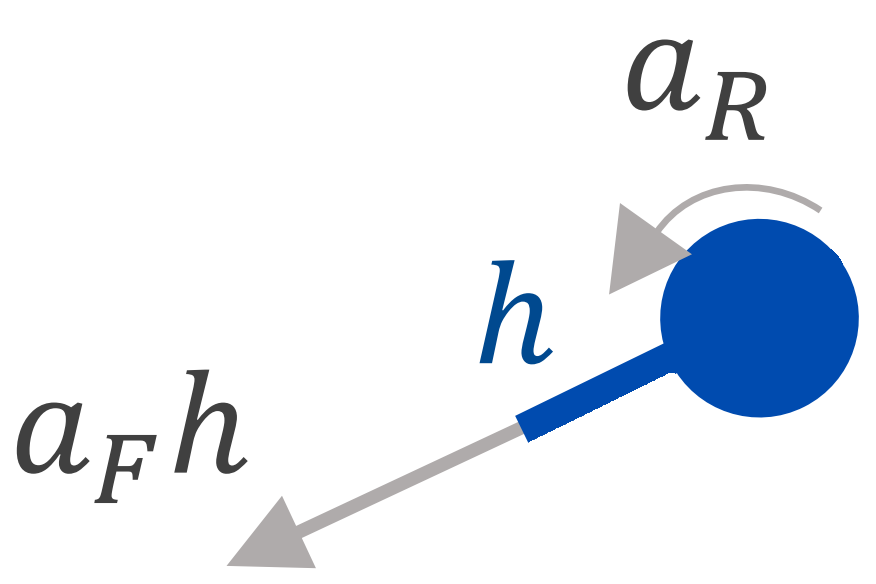
\includegraphics[width=\textwidth]{agent_active.png}
        %\caption{Active forces.}
        %\label{fig:image1}
    \end{minipage}
    \begin{minipage}{0.25\textwidth}
        \centering
        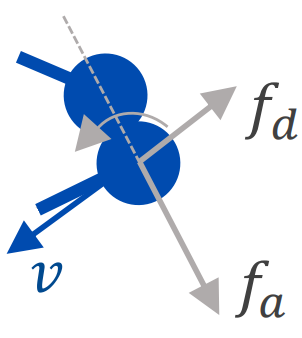
\includegraphics[width=\textwidth]{agent_passive.png}
        %\caption{Passive forces.}
        %\label{fig:image2}
    \end{minipage}
    \caption{Active (left) and passive (right) agent forces. \cite{li2023predator}}
    \label{fig:main_figure}
\end{figure}

Each timestep, the simulation updates the agents' positions and velocities based on the sum of forces acting on them.  
These can be summed up as:  

$$ \dot{x} = v $$  
$$ \dot{v} = \frac{ha_F + F_d + F_a}{m} $$  
$$ \dot{\theta} = a_R $$  

Where:
\begin{itemize}
    \item $x \in \mathbb{R}^2$ is the agent's position,
    \item $v \in \mathbb{R}^2$ is the agent's velocity,
    \item $\theta \in [-\pi, \pi]$ is the agent's heading angle,
    \item $h \in \mathbb{R}^2$ is the unit vector representing the agent's heading direction, calculated as $h = [\cos(\theta), \sin(\theta)]^T$,
    \item $m \in \mathbb{R}$ is the agent's mass.\\
\end{itemize}

To align the simulation with ant-like movement rather than the smooth, bird-like flight patterns of the original framework, several parameters will require significant adjustments. In their current settings—such as drag coefficient, stiffness coefficient, maximum forward acceleration, and rotational acceleration—the parameters are optimized for smooth, continuous paths with limited turning sharpness and no halting, resembling bird flight. However, to better emulate the more abrupt, flexible movement characteristic of ants in a 2D bird's-eye view, we will modify these parameters. Specifically, we’ll increase rotational flexibility, reduce constraints on movement continuity, and adjust stopping behaviors to allow agents more freedom in directional shifts and pauses.

\subsection{Model Performance Measures}

To see if any social distancing patterns emerge, we will transform the agent interactions into a network and analyze the network structure, as shown in \cite{Stroeymeyt2018}. We will look at network statistics that affect disease transmission, such as modularity (-), clustering (-), network efficiency (+) and degree centrality (+). We will also measure the average distance between agents, which would indicate that the agents are avoiding each other. First, these will be measured in a network before a pathogen is introduced to see the passive social distancing. Then we will introduce the pathogen and see how the network changes.

Other than that, emergent social distancing behavior should also be quite obvious in the simulation visualization. We expect healthy agents to stay away from infected ones and vice versa. This can be clearly seen if we increase the density of agents in the environment, we should see infected agents get isolated, forming empty circles around them, while healthy agents fill the rest of the simulation space.

\section{Results}

No experiments have been run so far, so there are no results to showcase yet.

\section{Discussion}

No results to discuss or conclude yet.

\printbibliography

\end{document}
